\chapter{Die Struktur des Nukleons}
Nukleon ist ausgedehntes Objekt.\\
Radius $\sim \mc{O}(\mr{fm})$. Untersuchung in Lepton-Nukleon-Streuung:
\begin{align*}
ep, \ \mu p , \ \nu(\bar{\nu}) p, eA, \mu A, \nu(\bar{\nu}) A
\end{align*}
Im Folgenden wird die Elektron-Proton-Streuung betrachtet.

Energieskala: $\Delta p \, \Delta x > \hbar \ \Ra \ E \gtrsim 1$\,GeV mit $\Delta p = \labs \vec{q}\rabs$ und $\Delta x = R_N < 1$\,fm\\
Typisch für $E$ sind $1 \dots 400$\,GeV

Bei HERA (DESY, Hamburg) ep-Kollisionen. Entspr. 50\,TeV Strahlenenergie in Fixed-Target-Experiment

\section{eN-Streuung -- Kinematik und WQ}
hier: QM (statt QFT nötig $\Ra$ Näherungen), Schrödingergleichung (obwohl relativistische Kinematik)

\begin{itemize}
\item \tb{Kinematik}\\
\begin{figure}[!ht]\centering
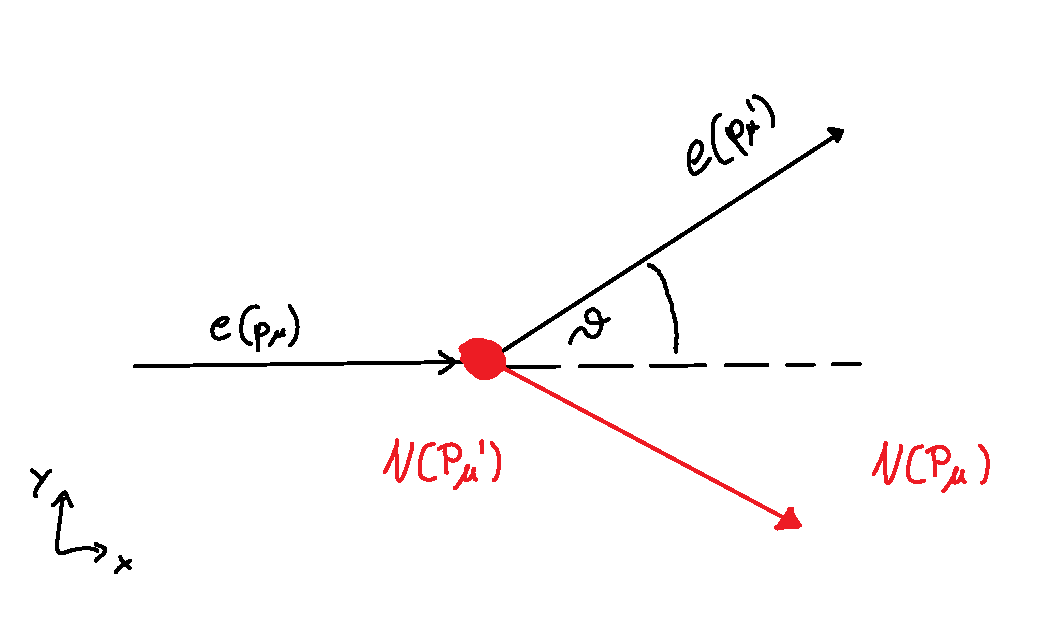
\includegraphics[width=.6\textwidth]{imgs/ep5-fig-6-1.pdf}
\caption{Elektron-Nukleon-Streuung \label{fig:6.1}}
\end{figure}
\begin{align}
\begin{split}
p_\mu = (E,p,0,0)\\
p_\mu^\prime = \lb E^\prime, p^\prime \cos \vartheta,  p^\prime \sin \vartheta,0 \rb \\
P_\mu = (M,0,0,0)
\end{split}
\end{align}
$E$- und $p$-Erhaltung:
\begin{align}
\begin{split}
\lb  p_\mu + P_\mu\rb ^2 = \lb p_\mu^\prime + P_\mu^\prime\rb ^2\\
\Ra \underbrace{p_\mu^2 + P_\mu^2 }_{m^2+M^2} + 2p_\mu P^\mu = \underbrace{{p_\mu^\prime}^2 + {P_\mu^\prime}^2}_{m^2+M^2} + 2p_\mu^\prime P^{\mu\prime}\
\Ra p_\mu P^\mu = p_\mu^\prime \lb  p^\mu + P^\mu - p^{\mu\prime}\rb \\
\Ra EM = \underbrace{p_\mu^\prime p^\mu}_{EE^\prime - pp^\prime \cos \vartheta} + E^\prime M - m^2
\end{split}
\end{align}
\begin{align}
\begin{split}
\boxed{E^\prime = E - \underbrace{\frac{EE^\prime - pp^\prime \cos \vartheta - m^2}{M}}_{>0, \text{ klein wenn } M\gg E}}
\end{split}
\end{align}
\begin{enumerate}
\item Wenn $M\gg E$ $\Ra$ $E^\prime = E$ (Rutherford, eN bei $E\sim 10$\,MeV)
\item Wenn $m\ll E$ $\Ra$ $E=p,\ E^\prime = p^\prime$
\begin{align}
\begin{split}
\Ra \boxed{E^\prime = \frac{E}{1 + \frac{E}{M}\lb  1- \cos \vartheta\rb }}
\end{split}
\end{align}
(eN-Streuung bei $E \gtrsim 10$\,MeV)
\end{enumerate}
\item \tb{Potentialstreuung}\\
Fall (1): $M \gg E$, \glqq kein\grqq{} E-Übertrag auf N
\begin{itemize}
\item[$\Ra$] Wie Streuung in ortsfestem Potential $V\lb \vec{r}\rb $ \\$\ra$ Hamiltonian $\Ham\lb \vec{r}\rb $
\begin{figure}[!ht]
\centering
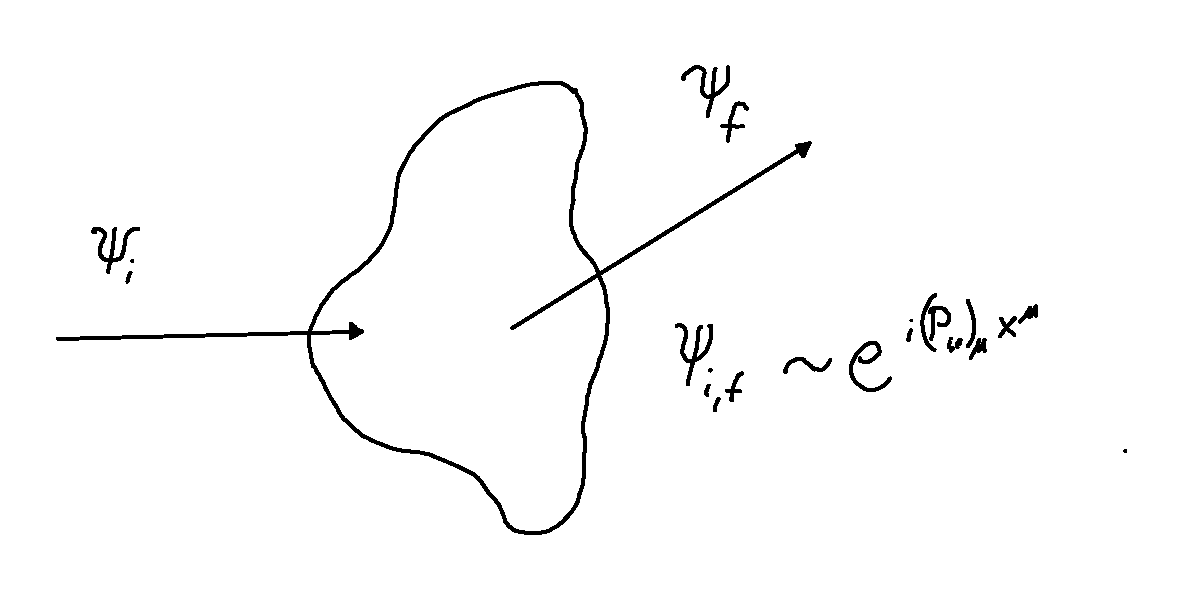
\includegraphics[width=.6\textwidth]{imgs/ep5-fig-6-2.pdf}
\caption{Veranschaulichung des Hamiltonian als WW-Operator\label{fig:6.2}}
\end{figure}
\item[$\Ra$] Nutze: \begin{compactitem}
\item QM-Störungsrechnung
\item Fermis Goldene Regel
\item Zustandsdichte im Endzustand
\end{compactitem}
\begin{align}
\Ra \boxed{ \Pa \sigma = \frac{{E^\prime}^2}{\lb  2\pi\rb ^2} \labs \int \Pa^3 r e^{i \vec{q}\vec{r}} \Ham\lb \vec{r}\rb  \rabs^2 \Pa \Omega }
\end{align}
\begin{compactitem}
\item[mit] $\vec{q} = \vec{p}-\vec{p}^\prime$
\item[] $\Ham\lb \vec{r}\rb  = (-e) V_A\lb \vec{r}\rb $
 \item[] $V_A$ als Coulombpotential des Targets
\end{compactitem}
$V_A\lb \vec{r}\rb $ wird von Ladungsdichte $\rho_A\lb \vec{r}\rb $ erzeugt\\
$\rho_A\lb \vec{r}\rb  = e f_A\lb \vec{r}\rb $ mit $\int \Pa^3 r f_A\lb \vec{r}\rb  = 1$\\
Somit die Poissongleichung (Elektrostatik)
\begin{align}
\boxed{\Lap V_A\lb \vec{r}\rb  = - \frac{\rho_A\lb \vec{r}\rb }{\epso} = -\frac{e}{\epso}f_A\lb \vec{r}\rb }
\end{align}
\begin{align*}
& \Ra \int \Pa^3 r e^{i \vec{q}\vec{r}} \Ham \lb \vec{r}\rb \\
&\qquad \labs\ \Lap e^{i \vec{q}\vec{r}} = - \labs \vec{q}\rabs^2 e^{i \vec{q}\vec{r}} \rno\\
& =  - \int \Pa^3 r \frac{1}{\labs\vec{q}\rabs^2} \lb  \Lap e^{i \vec{q}\vec{r}}\rb  \Ham\lb \vec{r}\rb \\
&\qquad \labs\ \text{2-fache partielle Integration} \rno \\
& = -\frac{1}{\labs \vec{q}\rabs ^2} \int \Pa^3 r e^{i\vec{q}\vec{r}} \underbrace{\lb  \Lap \Ham \lb \vec{r}\rb \rb }_{-e \frac{-\rho_A \lb \vec{r}\rb }{\epso}}\\
& = - \underbrace{\frac{e^2}{\labs \vec{q}\rabs^2 \epso}}_{=\frac{4\pi\alpha}{\labs \vec{q}\rabs^2}} \underbrace{\int \Pa^3 r e^{i\vec{q}\vec{r}} f_A\lb \vec{r}\rb }_\text{= Formfaktor $F\lb \vec{q}\rb $}
\end{align*}
Für punktförmiges Target:
\begin{align}
f_A \lb  \vec{r}\rb  = \delta \lb  \vec{r}\rb  \ \Ra \ F\lb \vec{q}\rb  \equiv 1,
\end{align}
also
\begin{align}
\boxed{ \begin{matrix}
\frac{\Pa \sigma}{\Pa \Omega} & = \frac{{E^\prime}^2}{\lb 2\pi\rb ^2} \labs \int \Pa^3 r e^{i\vec{q}\vec{r}}\Ham\lb \vec{r}\rb  \rabs^2\\
& = \frac{4 \alpha^2}{\labs \vec{q}\rabs^4}{E^\prime}^2 = \lno \frac{\Pa \sigma}{\Pa \Omega}\rabs_\text{Rutherford}
\end{matrix} }
\end{align}
Hierbei eigentlich: Faktor $Z_e^2 Z_p^2$

Erinnerung:
\begin{align}
\labs \vec{q}\rabs ^2 = \labs \vec{p} - \vec{p}^\prime \rabs^2 \overset{p= p^\prime}{=} 2 p^2 - 2p^2 \cos \vartheta = 4 p^2 \sin^2 \frac{\vartheta}{2}\nonumber \\
p^2 \llb \begin{matrix}
E_{kin} \cdot 2m & \text{nicht-relativistisch (Rutherford)}\\ EE^\prime & \text{relativistisch } (E \approx E^\prime = p)
\end{matrix} \rno \nonumber\\
\Ra \boxed{ \lno \frac{\Pa \sigma^\mathrm{eN}}{\Pa \Omega}\rabs _\mathrm{Rf} = \frac{Z_e^2 Z_p^2 \alpha^2 }{4 E^2 \sin^4 \frac{\vartheta}{2}} }
\end{align}
\end{itemize}
\item \tb{Korrekturen}
\begin{itemize}
\item[$\ra$] Ausgedehntes Target:
\begin{align}
\frac{\Pa \sigma}{\Pa \Omega} = \lno \frac{\Pa \sigma}{\Pa \Omega}\rabs_\mathrm{Rf} \cdot \labs F\lb  \vec{q} \rb  \rabs ^2
\end{align}
\item[$\ra$] Rückstoß-Korrektur (Energieübertrag)
\begin{align}
\frac{\Pa \sigma}{\Pa \Omega} = \lno \frac{\Pa \sigma}{\Pa \Omega}\rabs_\text{Rf} \frac{E^\prime}{E}
\end{align}
\item[$\ra$] Magnetisches Moment des $e^-$ (ohne magn. Moment des $N$)
\begin{align}
\frac{\Pa \sigma}{\Pa \Omega} = \lno \frac{\Pa \sigma}{\Pa \Omega}\rabs_\text{Rf} \cdot \lb  1 - \beta_e^2 \sin^2 \frac{\vartheta}{2}\rb 
\end{align}
für $\beta_e \ \ra \ 1$ (relativistisches $e^-$):
\begin{align*}
1-\beta_e^2 \sin^2\frac{\vartheta}{2} \ \ra \ \cos^2 \frac{\vartheta}{2}
\end{align*}
\item[$\Ra$] Rückstreuung ($\vartheta = 180^\circ$) unterdrückt\\
Grund: Helizitätserhaltung (folgt aus relativistischer QM für $\beta_e \ra 1$)
\begin{align*}
\text{Helizität} =  \frac{\vec \sigma \vec{p}}{\labs \vec{\sigma}\rabs \labs \vec{p} \rabs}
\end{align*}
\begin{align}
\boxed{ \frac{\Pa \sigma}{\Pa \Omega} = \frac{Z_e^2 Z_p^2 \alpha^2 }{4 E^2 \sin^4 \frac{\vartheta}{2}} \frac{E^\prime}{E} \cdot \cos^2 \frac{\vartheta}{2} = \lno \frac{\Pa \sigma}{\Pa \Omega}\rabs_\mathrm{Mott} }\\
\text{zusätzlich } \labs F\lb \vec{q}\rb  \rabs^2
\end{align}
\item[$\ra$] Magnetisches Moment des Targets (punktförmiges Dirac-Teilchen)
\begin{align}
\boxed{ \frac{\Pa \sigma}{\Pa \Omega} \ra \lno \frac{\Pa \sigma}{\Pa \Omega}\rabs_\mathrm{Mott}  \lb  1 + 2 \tau \tan^2 \frac{\vartheta}{2}\rb  }
\end{align}
\begin{compactitem}
\item[mit] $\tau = \frac{Q^2}{4 M^2} = \frac{- q_\mu q^\mu}{4 M^2}$
\end{compactitem}
Jetzt: Spin-Flip von Target möglich, $\lno \nicefrac{\Pa \sigma}{\Pa \Omega} \rabs_{\vartheta = 180^\circ} > 0$
\end{itemize}
\end{itemize}

\section{Elastische eN-Streuung}
N ist \tb{nicht} punktförmig $\Ra$ Formfaktor\\
\tb{2} Formfaktoren
\begin{compactitem}
\item $G_E\lb q^2\rb  \ra $ Verteilung der Ladung
\item $G_M\lb q^2\rb  \ra $ Verteilung der magnetischen Momente
\end{compactitem}
\begin{itemize}
\item[$\Ra$] WQ ist (nach Rosenbluth-Formel)
\begin{align}
\boxed{ \frac{\Pa \sigma}{\Pa \Omega} = \lno \frac{\Pa \sigma}{\Pa \Omega} \rabs_\mr{Mott} \lsb  \frac{G_E^2 +\tau \cdot G_M^2}{1 + \tau} + 2 \tau G_M^2 \tan^2 \frac{\vartheta}{2} \rsb  }
\end{align}
\item[$\ra$] Messung von $\frac{\Pa \sigma}{\Pa \Omega}\lb q^2\rb $ ergibt $G_{E,M}$
\begin{align}
\boxed{
G_{E,M}^p \lb Q^2\rb  = \frac{G_{E,M}^p \lb 0\rb }{\lb  1+ \frac{Q^2}{0.71\,\mr{GeV}^2}\rb ^2}
}
\end{align}

Auch:
\begin{align}
G_M^n = \frac{G_M^n \lb  0\rb }{\lb 1+ \frac{Q^2}{0.71\,\mr{GeV}^2}\rb ^2}
\end{align}
\item[$\Ra$] Ladungsverteilung
\begin{figure}[!ht]
\centering
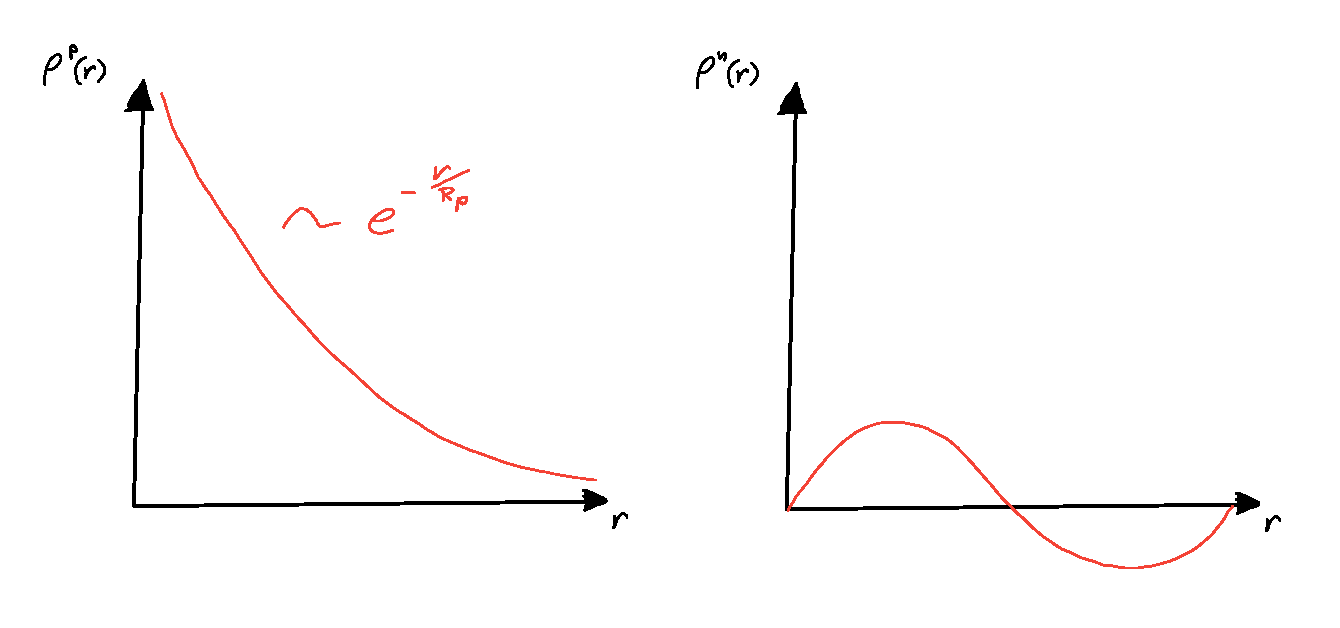
\includegraphics[width=.5\textwidth]{imgs/ep5-fig-6-3.pdf}
\caption{Ladungsverteilung eines Protons\label{fig:6.3}}
\end{figure}

Es gilt hierbei: $R_p \approx 0.86$\,fm
\item[$\ra$] $G_{M,E} \lb  Q^2 = 0\rb $ ist Ladung bzw. magnetisches Moment des Nukleons
\begin{align*}
\begin{matrix}
G_E^p(0) = 1 & \text{Ladung 1}e\\
G_E^n(0) = 0 & \text{Ladung 0}e\\
G_M^p(0) = 2.79 & \text{magnetisches Moment }\mu_p= 2.79\frac{e\hbar}{2M_p}\\
G_M^n(0) = -1.91 & \mu_n = - 1.91\frac{e\hbar}{2M_n}
\end{matrix}
\end{align*}
\end{itemize}

\section{Anregungszustände der Nukleonen}
Inelastische Streuung:
\begin{figure}[!ht]
\centering
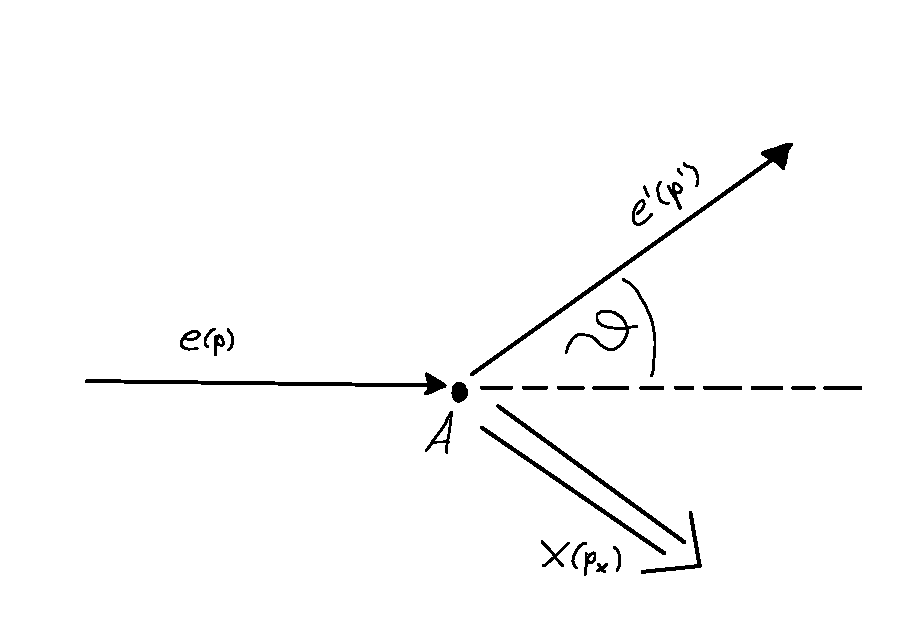
\includegraphics[width=.6\textwidth]{imgs/ep5-fig-6-4.pdf}
\caption{Skizze zur inelastischen Streuung eines $e^-$ an einem Teilchen A\label{fig:6.4}}
\end{figure}
Aus \autoref{fig:6.4}
\begin{align*}
q_\mu = p_\mu - p_\mu^\prime\\
p_{X,\mu} = p_{A,\mu} + q_\mu
\end{align*}
Es gilt also somit:
\begin{align}
\begin{split}
\underbrace{p_X^2}_{W^2} = \underbrace{p_A^2}_{M_A^2} + \underbrace{q_\mu q^\mu}_{-Q^2} + \underbrace{2 p_{A,\mu}q^\mu}_{2M_A\lb E-E^\prime\rb =2 M\nu}\\
\Ra W^2 = -Q^2 + M^2 + 2 \nu M = Q^2 \lsb  \frac{2 \nu M}{Q^2} -1 \rsb  +M^2\\
\frac{2\nu M}{Q^2} = \frac{1}{x}
\end{split}
\end{align}
$x$ = \glqq Bjorken-x\grqq
\begin{itemize}
\item[$\lt$] elastisch: $W^2 = M^2 \Ra x=1$
\item[$\lt$] inelastisch: $W^2 > M^2 \Ra x<1$
\item[$\lt$] $\boxed{2}$ Variablen erforderlich, um inelastische Kinematik festzulegen\\
$\lt$ $\lb x, Q^2\rb $, $\lb x, W\rb $, $\lb E^\prime, \vartheta\rb $
\item[$\Ra$] Messung von $\dfrac{\sigma}{W}$

\begin{figure}[!ht]
\centering
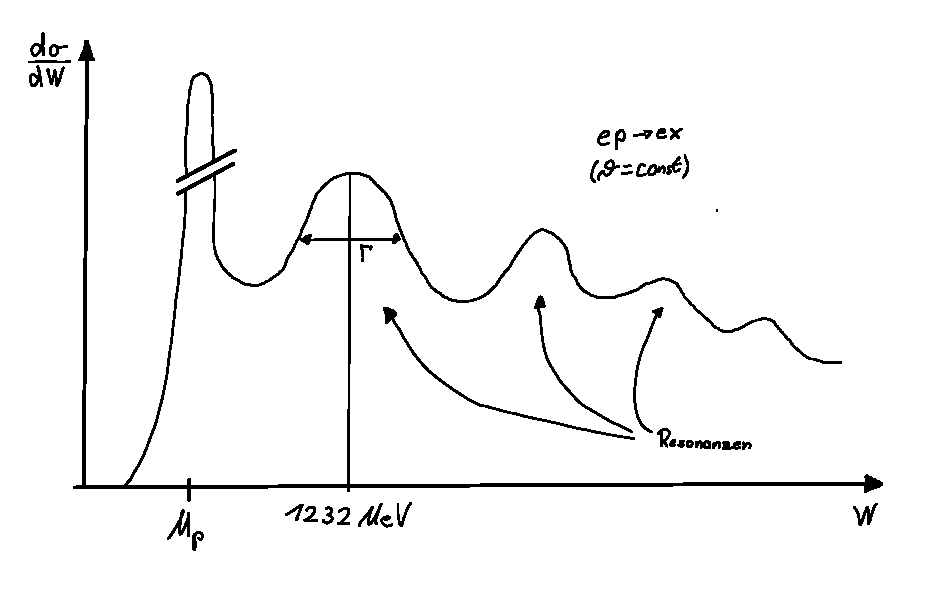
\includegraphics[width=.6\textwidth]{imgs/ep5-fig-6-5.pdf}
\caption{Resonanzpeaks der $eN$-Streuung\label{fig:6.5}}
\end{figure}

\item[$\ra$] Peaks = \glqq Resonanzen\grqq{}
\begin{compactitem}
\item[$\Ra$] kurzlebige Zustände
\item[$\Ra$] Nukleonanregungen
\item[$\Ra$] Prominent: $\Delta^+\lb 1232\rb $
\begin{align}
\begin{split}
M\lb \Delta^+\lb 1232\rb \rb  = 1.232\,\mr{GeV}\\
\Gamma_{\Delta^+} \approx 120\,\mr{MeV}
\end{split}
\end{align}
$\ra$ Lebensdauer des $\Delta^+\lb 1232\rb $:
\begin{align}
\tau = \frac{1}{\Gamma}= \frac{197\,\mr{\nicefrac{MeV}{fm}}}{120\,\mr{MeV}}\frac{1}{c} \approx 0.5\cdot 10^{-23} \,\mr s
\end{align}
$\tau$ ist typischer Wert für starke Wechselwirkung
\end{compactitem}
\item[$\lt$] Genauere Untersuchung:
\begin{align*}
\ket{\Delta^+\lb 1232\rb } = \ket{uud} \ \ \ \text{wie $p$}\\
J^p\lb \Delta^+\lb 1232\rb \rb  = \lb  \frac{3}{2}\rb ^+; \ \ \ J^p \lb p\rb  = \lb  \frac{1}{2}\rb  ^+
\end{align*}
\item[$\lt$] $\Delta$-Zerfall
\begin{figure}[!ht]
\centering
    \begin{tikzpicture}
        \begin{feynman}
            \vertex (a1) {$u$};
            \vertex[right=2cm of a1] (a2);
            \vertex[right=3cm of a1] (a3);
            \vertex[right=5cm of a1] (a4) {$u$};
            \vertex[below=2em of a1] (b1) {$u$};
            \vertex[right=2.5cm of b1] (b2);
            \vertex[right=5cm of b1] (b3) {$u$};
            \vertex[below=2em of b1] (c1) {$d$};
            \vertex[right=5cm of c1] (c2) {$d$};
            \vertex[above=2.667em of a4] (d1) {$\bar u$};
            \vertex[above=4em of a4] (e1) {$u$};
            
            \vertex[right=8cm of a1] (f1) {$u$};
            \vertex[right=2cm of f1] (f2);
            \vertex[right=3cm of f1] (f3);
            \vertex[right=5cm of f1] (f4) {$d$};
            \vertex[below=2em of f1] (g1) {$u$};
            \vertex[right=2.5cm of g1] (g2);
            \vertex[right=5cm of g1] (g3) {$u$};
            \vertex[below=2em of g1] (h1) {$d$};
            \vertex[right=5cm of h1] (h2) {$d$};
            \vertex[above=2.667em of f4] (i1) {$\bar d$};
            \vertex[above=4em of f4] (j1) {$u$};

            \diagram* {
            (a1) -- (a2) -- (e1),
            (a2) -- [gluon] (a3) -- (d1),
            (b1) -- (b3),
            (a3) -- (a4),
            (c1) -- (c2),
            
            (f1) -- (f2) -- (j1),
            (f2) -- [gluon] (f3) -- (i1),
            (g1) -- (g3),
            (f3) -- (f4),
            (h1) -- (h2),
            };
            \draw [decoration={brace}, decorate] (c1.south west) -- (a1.north west)
            node [pos=0.5, left] {$\Delta^+$};
            \draw [decoration={brace}, decorate] (a4.north east) -- (c2.south east)
            node [pos=0.5, right] {$p$};
            \draw [decoration={brace}, decorate] (e1.north east) -- (d1.south east)
            node [pos=0.5, right] {$\pi^0$};

            \draw [decoration={brace}, decorate] (h1.south west) -- (f1.north west)
            node [pos=0.5, left] {$\Delta^+$};
            \draw [decoration={brace}, decorate] (f4.north east) -- (h2.south east)
            node [pos=0.5, right] {$n$};
            \draw [decoration={brace}, decorate] (j1.north east) -- (i1.south east)
            node [pos=0.5, right] {$\pi^+$};
        \end{feynman}
    \end{tikzpicture}
\caption{Zerfallsgrafiken für $\Delta^+$ zu p bzw. n}
\end{figure}
\end{itemize}

\section{Tiefinelastische Streuung}
Frage: Was passiert bei höheren Energien?\\
Erwartung: Bessere räumliche Auflösung $\Ra$ Bestandteile des Nukleons
\begin{itemize}
\item Beobachtung 1\\
Bei $W \gtrsim 2.5$\,GeV: Kontinuum von hadronischen Endzuständen
\begin{itemize}
\item[$\lt$] keine Resonanzen
\item[$\lt$] unterschiedliche Hadronenkombinationen
\item[$\lt$] Differentieller WQ hängt von zwei Variablen ab, z.B.
\begin{align*}
\underbrace{Q^2 = - q_\mu q^\mu; \ \ \ x = \frac{Q^2}{2M\nu} = \frac{- q_\mu q^\mu}{2 P_{A,\mu}q^\mu}}_\text{Lorentz-Invariant}
\end{align*}
\item[$\lt$] Darstellung des WQ:
\begin{align}
\dfrac{^2 \sigma}{\Omega \Pa E^\prime} = \lno \dfrac{\sigma}{\Omega}\rabs_\mr{Mott} \lb  W_2\lb x, Q^2\rb  + 2 W_1 \lb x, Q^2\rb  \tan^2 \frac{\vartheta}{2}\rb  
\end{align}
\begin{compactitem}
\item[mit] $W_2\lb x, Q^2\rb $: Ladungs-WW
\item[] $2 W_1 \lb x, Q^2\rb  \tan^2 \frac{\vartheta}{2}$: magnetische WW
\item[] $W_{1,2}$: \tb{\glqq Strukturfunktion\grqq}
\end{compactitem}
Achtung:
\begin{align*}
\underbrace{G_{E,M}\lb Q^2\rb }_\text{elastisch} \ \longrightarrow \ \underbrace{W_{1,2} \lb  x, Q^2\rb }_\text{tiefinelastisch}
\end{align*}
\item[$\lt$] Dimensionslose Strukturfunktionen:
\begin{align}
F_2\lb x, Q^2\rb  = \nu W_2 \lb x, Q^2\rb \\
F_1 \lb x, Q^2\rb  = MW_1 \lb  x, Q^2\rb 
\end{align}
\end{itemize}
\item Beobachtung 2\\
Erste Messungen 1968 ff.
\begin{itemize}
\item[$\Ra$] $F_2\lb  x, Q^2\rb $ hängt (nur sehr schwach) von $Q^2$ ab (\glqq Skaleninvarianz\grqq)
\item[$\Ra$] Interpretation: $Q^2$-Abhängigkeit aus Fourier-Transformation um $\rho (\vec r)$
\begin{itemize}
\item[$\Ra$] $\rho \lb \vec{r}\rb  = \delta \lb  \vec{r}\rb $
\item[$\Ra$] Streuung an \tb{punktförmigen} Teilchen (Konstituenten des Nukleons)
\item[$\Ra$] \tb{Quarks!} Bewegen sich \glqq quasi-frei\grqq{} im Nukleon
\end{itemize}
\item[$\ra$] Kinematik
\begin{figure}[!ht]
\centering
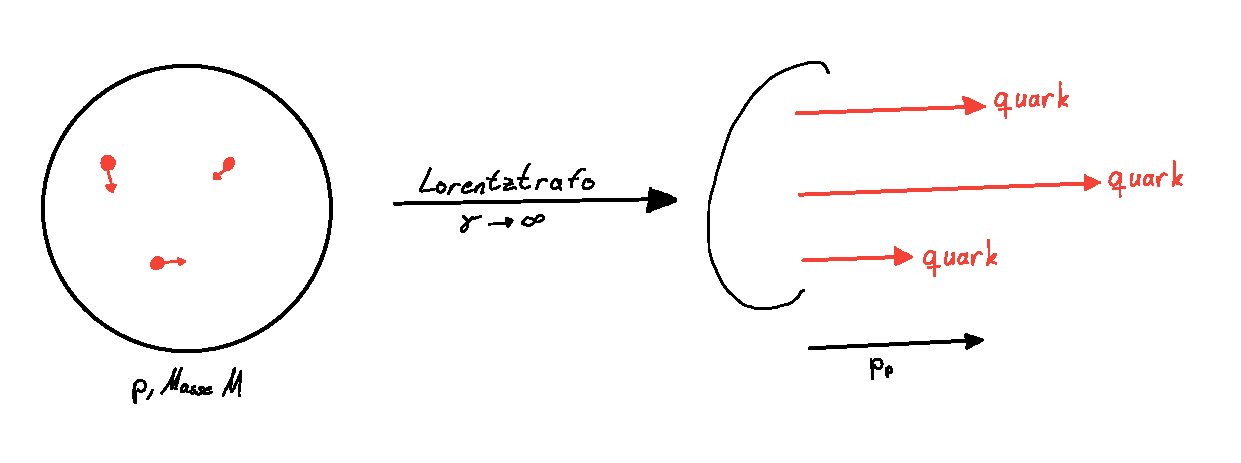
\includegraphics[width=.6\textwidth]{imgs/ep5-fig-6-7.pdf}
\caption{Strukturskizze eines Protons\label{fig:6.7}}
\end{figure}

\ni Aus \autoref{fig:6.7}: alle Massen und Transversalimpulse sind vernachlässigbar\\
Quark-Impuls:
\begin{align}
p_i = \xi_i p_p= \xi_i \lb \gamma M , \gamma M, 0, 0\rb 
\end{align}

\item[$\lt$] ep-Streuung $\hat{=}$ elastische eq-Streuung

\begin{figure}[!ht]
\centering
    \begin{tikzpicture}
        \begin{feynman}
            \vertex (a1);
            \vertex[right = 3cm of a1] (a2);
            \vertex[above right = 3cm of a2] (b1);
            \vertex[below right = 3cm of a2] (c1);
            
            \diagram*{
            (a1) -- [fermion, edge label = $q_i(p_i)$] (a2),
            (a2) -- [boson, edge label = $\gamma(q)$] (b1),
            (a2) -- [fermion, edge label = $q_f(p_f)$] (c1),
            };
        \end{feynman}
    \end{tikzpicture}
\caption{Feynmandiagramm zur Quarkstreeung\label{fig:6.8}}
\end{figure}

\begin{align}
p_f^2 = \lb  p_i + q\rb ^2 =p_i^2 - Q^2 + 2p_{i_\mu}q^\mu \nonumber \\
2p_{i,\mu} q^\mu = 2 \xi_i p_{p,\mu} q^\mu \overset{!}{=}Q^2 \nonumber\\
\boxed{ \xi_i = \frac{Q^2}{2 p_{i,\mu}q^\mu} = \frac{Q^2}{2 M \nu} = x }
\end{align}
\item[$\Ra$] $x=$ Anteil an p-Impuls, den das getroffene Quark trägt!
\end{itemize}
\item Beobachtung 3\\
$F_{1,2} \lb x, Q^2\rb  \approx F_{1,2}\lb x\rb $ ergeben \glqq Quark-Dynamik im Nukleon\grqq{}\\
Vereinfacht:
\begin{align}
\boxed{ \sigma \lb  e, p \rb   = \sum_{q \in p } \sigma \lb eq_i \rb   q_i\lb x\rb }
\end{align}
\begin{compactitem}
\item[mit] $q_i(x)$: \glqq Parton-Verteilungsfunktion\grqq{} (PDF)
\item[] $\sigma \lb ep\rb , \ \sigma\lb eq_i\rb $: eigentlicher differentieller WQ
\end{compactitem}
\tb{\glqq Parton\grqq}: Quark oder Gluon\\
für $q_i$ mit $x$ im Parton:
\begin{align}
\boxed{q_i\lb x\rb  = \dfrac{\lb WS\rb }{x}}
\end{align}
\end{itemize}

\vorlesung{12. Januar 2018}

\begin{figure}[!ht]
\centering
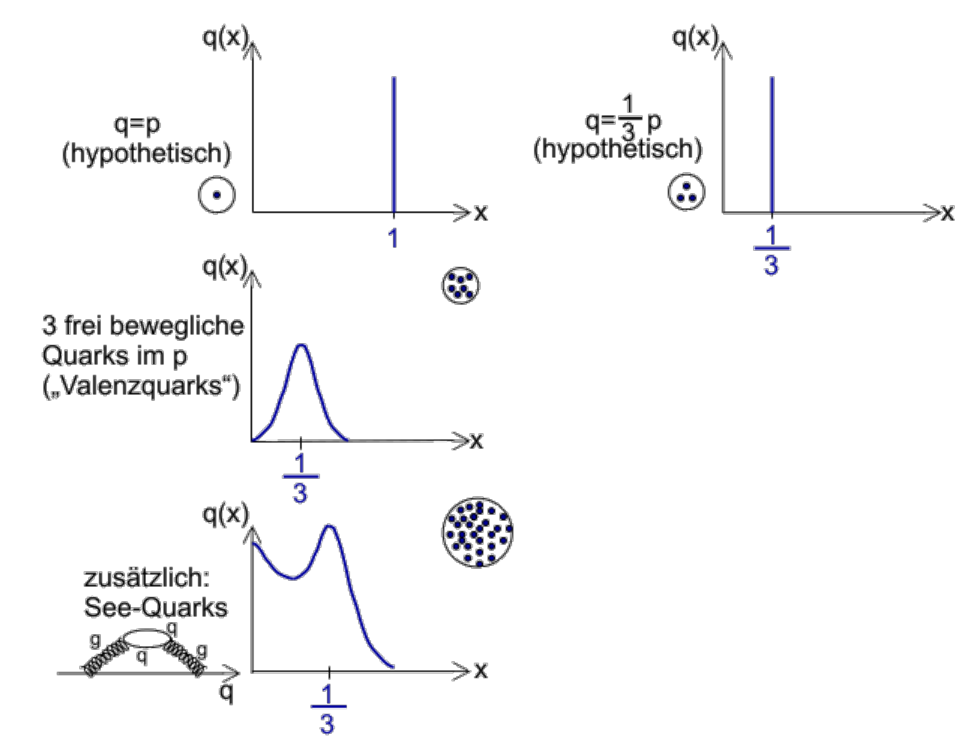
\includegraphics[width=.9\textwidth]{imgs/ep5-fig-6-9.pdf}
\caption{Erwartete Verteilungen für $q_i(x)$\label{fig:6.9}}
\end{figure}
\begin{itemize}
\newpage
\item \tb{Beobachtung 4}\\
$F_1$-Term im WQ kommt vom magnetischen Moment des Targets
\begin{itemize}
\item[$\Ra$] Erwartung:
\begin{align}
F_1\lb  x, Q^2\rb  = \begin{cases}0, \text{ wenn Spin}(q) = 0\\ 
\frac{F_2\lb x, Q^2\rb }{2x}, \text{ wenn Spin}(q) = \frac{1}{2} \end{cases}
\end{align}
\item[$\Ra$] Messung (Callen-Gross-Relation):
\begin{align}
\boxed{ 2xF_1\lb x, Q^2\rb  = F_2 \lb  x, Q^2\rb  }
\end{align}
$\ra$ Quarks sind Fermionen
\end{itemize}
\item \tb{Beobachtung 5}
\begin{align}
\int_0^1 \sum_{q\text{ in } p} x q_i(x) \Pa x \approx 0.5 \neq 1
\end{align}
1 erwartet, wenn nur Quarks q im Proton p wären.\\
$\Ra$ weitere Partonen = Gluonen in p
\newpage

\item \tb{Beobachtung 6}\\
Skaleninvarianz ist verletzt $\Ra$ Effekt der starken WW

\begin{figure}[!ht]
\centering
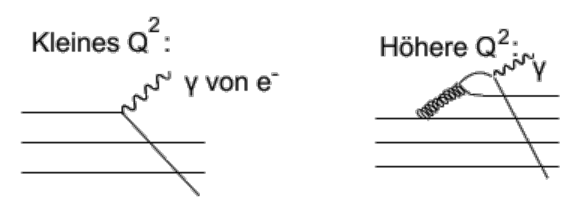
\includegraphics[width=.6\textwidth]{imgs/ep5-fig-6-10.pdf}
\caption{Verschiebung der Partonen-Verteilung mit zunehmenden $Q^2$ zu kleinen $x$\label{fig:6.10}}
\end{figure}
\end{itemize}
